\documentclass{article}
\usepackage{v-equation}
\usepackage{pgfplots}
\geometry{
paperwidth=5in, 
paperheight=5in, 
top=10mm, 
bottom=10mm, 
left=10mm, 
right=10mm
}

\begin{document}
\begin{center}
Bragg’s law
\end{center}
\vspace*{\fill}
\begin{center}
\begin{tikzpicture}
	\coordinate (A) at (-2, 1.2);
	\coordinate (AX) at (-2, 0);
	\coordinate (O) at (0, 0);
	\coordinate (B) at (2, 1.2);
	\coordinate (BX) at (2, 0);
	\foreach \x in {-3, -2, ..., 3}{
	\foreach \y in {0, -1, ..., -3}{
	\tzline[dashed](-3, \y)(3, \y)
	\tzdot*(\x, \y)(4pt)
	}
	}
	
	\tzline[-->--=0.4](A)(O)
	\tzline[-->--=0.6](O)(B)
	\tzanglemark(A)(O)(AX){$\theta$}(15pt)
	\tzanglemark(BX)(O)(B){$\theta$}(15pt)
	\tzline[|<->|]<-0.5, 0>(-3, -1)(-3, -2){$d$}[l, midway]
	\tznode<0, -3.65>(0, 0){X-rays incident on a crystal}
\end{tikzpicture}
\end{center}
\vspace*{\fill}
{\LARGE{
\begin{align*}
2d \sin \theta = n\lambda
\end{align*}
}}
\vspace*{\fill}

\pagebreak
\vspace*{\fill}
\begin{align*}
d &- \texttt{inter-atomic distance}\\
\theta &- \texttt{angle of incidence}\\
n &- \texttt{1, 2, 3, ...}\\
\lambda &- \texttt{wavelength of X-rays}
\end{align*}

\vspace*{\fill}

\begin{center}
	\fbox{\qrcode[link, height=2cm]{https://drive.google.com/drive/folders/16f38R9EjxZPGiPzMUPzpNHR_IG_zddxT?usp=share_link}}
\end{center}

\end{document}
